% !TEX root = ../CourseOT.tex

%%%%%%%%%%%%%%%%%%%%%%%%%%%%%%%%%%%%%%%%%%%%%%%%%%%%%%%%%%%%%%%%%%%%%%%%%%%
%%%%%%%%%%%%%%%%%%%%%%%%%%%%%%%%%%%%%%%%%%%%%%%%%%%%%%%%%%%%%%%%%%%%%%%%%%%
%%%%%%%%%%%%%%%%%%%%%%%%%%%%%%%%%%%%%%%%%%%%%%%%%%%%%%%%%%%%%%%%%%%%%%%%%%%
\section{Kantorovitch Relaxation}

%%%%%%%%%%%%%%%%%%%%%%%%%%%%%%%%%%%%%%%%%%%%%%%%%%%%%%%%%%%%%%%%%%%%%%%%%%%
\subsection{Discrete Relaxation}

\todo{reduce this + lack of symmetry}
The assignment problem has several limitations in practical settings, also encountered when using the Monge problem. Indeed, because the assignment problem is formulated as a permutation problem, it can only be used to compare two points clouds of the \emph{same} size. A direct generalization to discrete measures with non-uniform weights can be carried out using Monge's formalism of pushforward maps, but that formulation may also be degenerate it there does not exist feasible solutions satisfying the mass conservation constraint~\eqref{eq-monge-constr} (see the end of Remark~\ref{rem-monge1}). Additionally, the assignment Problem~\eqref{eq-monge-discr} is combinatorial, whereas the feasible set for the Monge Problem~\eqref{eq-monge-continuous}, consisting in all push-forward measures that satisfy the mass conservation constraint, is \emph{non-convex}. Both are therefore difficult to solve in their original formulation.


The key idea of~\cite{Kantorovich42} is to relax the deterministic nature of transportation, namely the fact that a source point $x_i$ can only be assigned to another, or transported to one and one location $T(x_i)$ only. Kantorovich proposes instead that the mass at any point $x_i$ be potentially dispatched across several locations. Kantorovich moves away from the idea that mass transportation should be ``deterministic'' to consider instead a ``probabilistic'' (or ``fuzzy'') transportation, which allows what is commonly known now as ``mass splitting'' from a source towards several targets. This flexibility is encoded using, in place of a permutation $\sigma$ or a map $T$, a coupling matrix $\P  \in \RR_+^{n \times m}$, where $\P_{i,j}$ describes the amount of mass flowing from bin $i$ (or point $x_i$) towards bin $j$ (or point $x_j$), 
$x_i$ towards $y_j$ in the formalism of discrete measures~\eqref{eq-pair-discr}. Admissible couplings admit a far simpler characterization than Monge maps:
\eql{\label{eq-discr-couplings}
	\CouplingsD(\a,\b) \eqdef \enscond{ \P \in \RR_+^{n \times m} }{
		\P \ones_m = \a \qandq 
		\transp{\P} \ones_n = \b	
	},
}
where we used the following matrix-vector notation
\eq{
	\P \ones_m = \left(\sum_j \P_{i,j}\right)_i \in \RR^n
	\qandq
	\transp{\P} \ones_n = \left(\sum_i \P_{i,j}\right)_j \in \RR^m. 
}
The set of matrices $\CouplingsD(\a,\b)$ is bounded, defined by $n+m$ equality constraints, and therefore a convex polytope (the convex hull of a finite set of matrices).

%
Additionally, whereas the Monge formulation (as illustrated in the right plot of Figure~\ref{fig-non-unique-matching}) was intrisically asymmetric, Kantorovich's relaxed formulation is always symmetric, in the sense that a coupling $\P$ is in  $\CouplingsD(\a,\b)$ if and only if  $\transp{\P}$ is in $\CouplingsD(\b,\a)$.

Kantorovich's optimal transport problem now reads
\eql{\label{eq-mk-discr}
	\MKD_{\C}(\a,\b) \eqdef 
	\umin{\P \in \CouplingsD(\a,\b)}
		\dotp{\C}{\P} \eqdef \sum_{i,j} \C_{i,j} \P_{i,j}. 
}
This is a linear program (see Chapter~\ref{c-algo-basics}), and as is usually the case with such programs, its solutions are not necessarily unique. 

%%%%%%%%%%
\paragraph{Linear programming algorithms}

Complexity of simplex $n^3 \log n$.
Interior points.


%%%%%%%%%%
\paragraph{Permutation Matrices as Couplings} 

TODO thm Birkof Von Neumann: extremal points, optim, demo (bipartite graph).

For a permutation $\si\in\Perm(n)$, we write $\P_{\si}$ for the corresponding permutation matrix,
	\eql{\label{eq-perm-matrices}
		\foralls (i,j) \in \range{n}^2, \quad
		(\P_{\si})_{i,j} = \choice{
			1/n \qifq j=\si_i, \\
			0 \quad\text{otherwise.} 
		}
	} 
One can check that in that case
\eq{\dotp{\C}{\P_{\si}}=\frac{1}{n}\sum_{i=1}^n \C_{i,\si_i},}
which shows that the assignment problem~\eqref{eq-optimal-assignment} can be recast as a Kantorovich problem~\eqref{eq-mk-discr} where the couplings $\P$ are restricted to be exactly permutation matrices:
\eq{\umin{\si \in \Perm(n)} \frac{1}{n}\sum_{i=1}^n \C_{i,\si(i)} = \umin{\si \in \Perm(n)} \dotp{\C}{\P_{\si}}.}
Next, one can easily check that the set of permutation matrices is strictly included in the so-called Birkhoff polytope $\CouplingsD(\ones_n/n,\ones_n,n)$. Indeed, for any permutation $\si$ we have $\P_{\si}\ones=\ones_n$ and $\transp{\P_{\si}}\ones=\ones_n$, whereas $\ones_n\transp{\ones_n}/n^2$ is a valid coupling but not a permutation matrix. Therefore, one has naturally that
$$ \umin{\si \in \Perm(n)} \dotp{\C}{\P_{\si}} \leq  \MKD_{\C}(\ones_n/n,\ones_n/n).$$

The following proposition shows that these problems result in fact in the same optimum, namely that one can always find a permutation matrix that minimizes Kantorovich's problem~\eqref{eq-mk-discr} between two uniform measures $\a=\b=\ones_n/n$, which shows that the Kantorovich relaxation is \emph{tight} when considered on assignment problems. %Note however that some computational algorithm, which are combinatorial in nature, are dedicated to the case of uniform histograms with the same number of points (see Chapter~\ref{c-algo-basics}). 
%
Figure~\ref{fig-matching-kantorovitch} shows on the left a 2-D example of optimal matching corresponding to this special case. 
%

\begin{figure}
\centering
\begin{tabular}{@{}c@{\hspace{5mm}}c@{}}
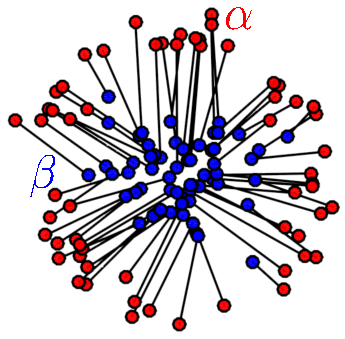
\includegraphics[width=.25\linewidth]{matching-kantorovitch/matching}&
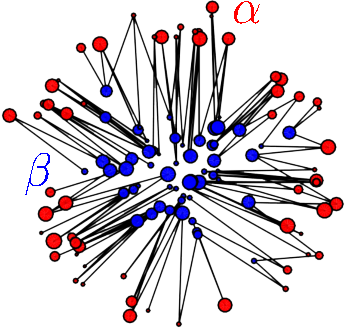
\includegraphics[width=.25\linewidth]{matching-kantorovitch/weighted}
\end{tabular}
\caption{\label{fig-matching-kantorovitch}
%
Comparison of optimal matching and generic couplings. A black segment between $x_i$ and $y_j$ indicates a non-zero element in the displayed optimal coupling $\P_{i,j}$ solving~\eqref{eq-mk-discr}.
%
Left: optimal matching, corresponding to the setting of Proposition~\eqref{prop-matching-kanto} (empirical measures with the same number $n=m$ of points).
%
Right: these two weighted point clouds cannot be matched; instead a Kantorovich coupling can be used to associate two arbitrary discrete measures.  
}
\end{figure}


\begin{prop}[Kantorovich for matching]\label{prop-matching-kanto}
	If $m=n$ and $\a=\b=\ones_n/n$, then there exists an optimal solution for Problem~\eqref{eq-mk-discr} $\P_{\si^\star}$, which is a permutation matrix associated to an optimal permutation $\si^\star \in \Perm(n)$ for Problem~\eqref{eq-optimal-assignment}.	
\end{prop}

\begin{proof}
	Birkhoff's theorem states that the set of extremal points of $\CouplingsD(\ones_n/n,\ones_n/n)$ is equal to the set of permutation matrices. A fundamental theorem of linear programming
	\cite[Theorem 2.7]{bertsimas1997introduction} 
	states that the minimum of a linear objective in a non-empty polyhedron, if finite, is reached at an extremal point of the polyhedron.
\end{proof}




%%%%%%%%%%%%%%%%%%%%%%%%%%%%%%%%%%%%%%%%%%%%%%%%%%%%%%%%%%%%%%%%%%%%%%%%%%%
\subsection{Relaxation for Arbitrary Measures}

TODO: Reminder on duality with continuous function.
  Radon measure: important to do duality and study optimization.


The definition of $\MK_\c$ in~\eqref{eq-kanto-discr} can be extended to arbitrary measures by considering couplings $\pi \in \Mm_+^1(\X \times \Y)$ which are joint distributions over the product space. The discrete case is a special situation where one imposes this product measure to be of the form $\pi = \sum_{i,j} \P_{i,j} \de_{(x_i,y_j)}$. In the general case, the mass conservation constraint~\eqref{eq-discr-couplings} should be rewritten as a marginal constraint on joint probability distributions
\eql{\label{eq-coupling-generic}
	\Couplings(\al,\be) \eqdef 
	\enscond{
		\pi \in \Mm_+^1(\X \times \Y)
	}{
		P_{\X\sharp} \pi = \al
		\qandq
		P_{\Y\sharp} \pi = \be
	}.
} 
Here $P_{\X\sharp}$ and $P_{\Y\sharp}$ are the push-forward (see Definition~\ref{defn-pushfwd}) by the projections $P_\X(x,y)=x$ and $P_\Y(x,y)=y$.
%
Figure~\ref{fig-settings} shows a schematic visualization of the coupling constraints for different class of problem (discrete measures and densities).
%
Using~\eqref{eq-equiv-pushfwd}, these marginal constraints are equivalent to imposing that $\pi(A \times \Y)=\al(A)$ and $\pi(\X \times B)=\be(B)$ for sets $A \subset \X$ and $B \subset \Y$.


\begin{figure}
\centering
\begin{tabular}{@{}c@{\hspace{5mm}}c@{\hspace{5mm}}c@{}}
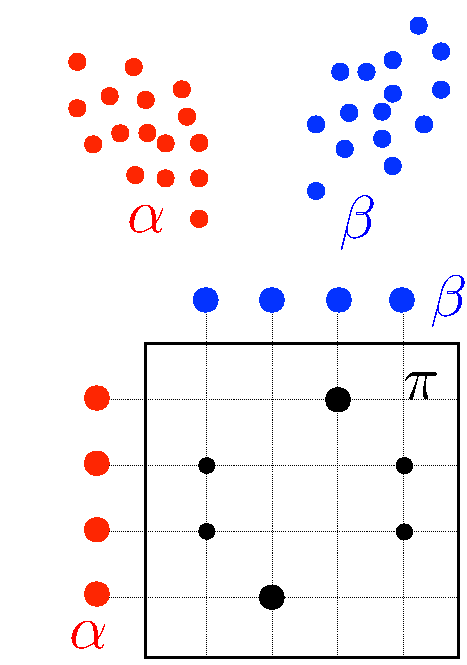
\includegraphics[width=.22\linewidth]{settings/discrete}&
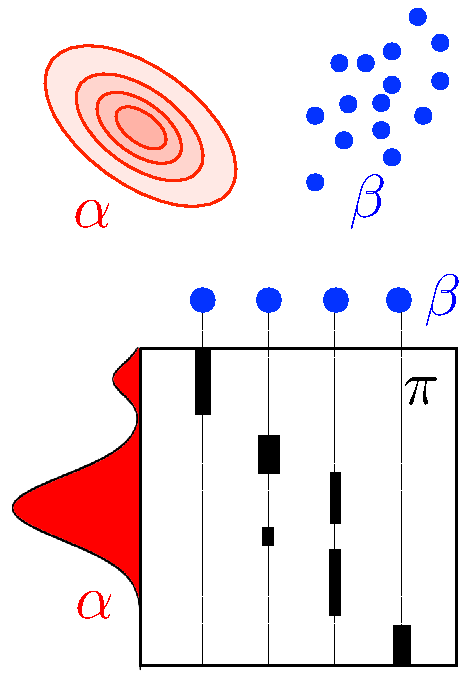
\includegraphics[width=.22\linewidth]{settings/semi-discrete}&
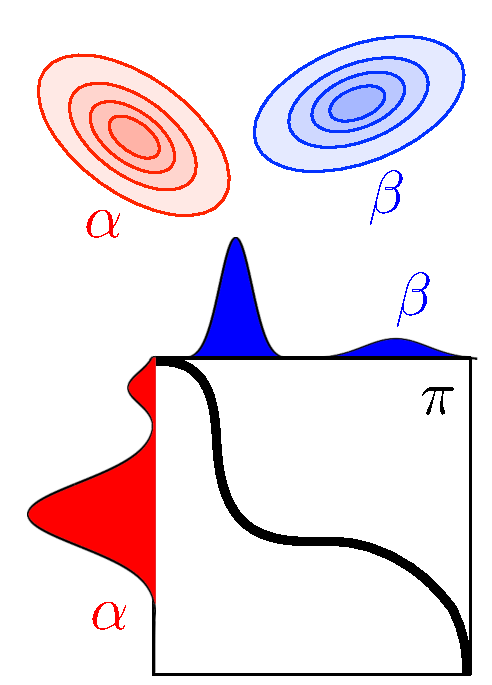
\includegraphics[width=.22\linewidth]{settings/continuous}\\
Discrete & Semi-discrete & Continuous
\end{tabular}
\caption{\label{fig-settings}
Schematic viewed of input measures $(\al,\be)$ and couplings $\Couplings(\al,\be)$ encountered in the three main scenario for Kantorovich OT. Chapter~\ref{c-algo-semidiscr} is dedicated to the semi-discrete setup.
}
\end{figure}



The Kantorovich problem~\eqref{eq-mk-discr} is then generalized as 
\eql{\label{eq-mk-generic}
	\MK_\c(\al,\be) \eqdef 
	\umin{\pi \in \Couplings(\al,\be)}
		\int_{\X \times \Y} \c(x,y) \d\pi(x,y).
}
This is an infinite-dimensional linear program over a space of measures. 
%
Figure~\ref{fig-couplings} shows examples of discrete and continuous optimal coupling solving~\eqref{eq-mk-generic}.
%
Figure~\ref{fig-couplings-simple} shows other examples of optimal 1-D couplings, involving discrete and continuous marginals.



\begin{figure}
\centering
\begin{tabular}{@{}c@{\hspace{10mm}}c@{}}
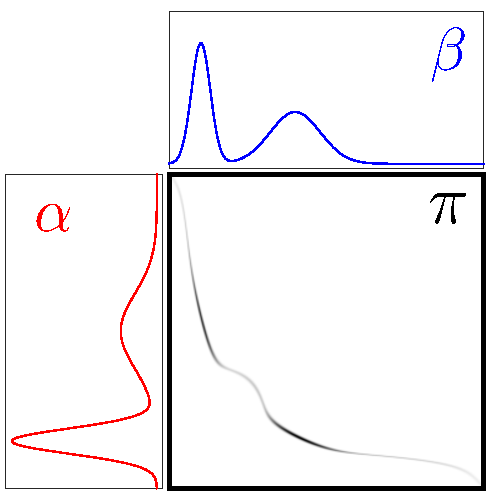
\includegraphics[width=.2\linewidth]{couplings/couplings-continuous}&
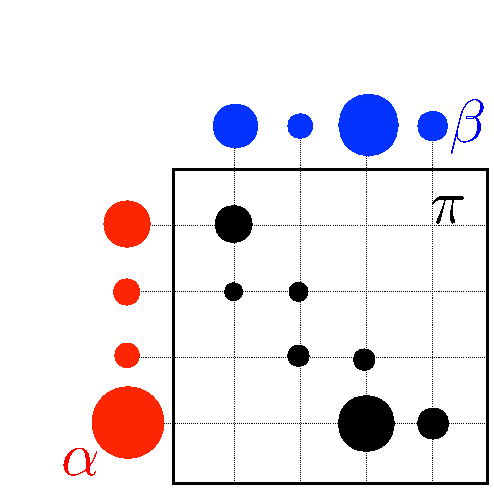
\includegraphics[width=.2\linewidth]{couplings/couplings-discr}
\end{tabular}
\caption{\label{fig-couplings}
Left: ``continuous'' coupling $\pi$ solving~\eqref{eq-coupling-generic} between two 1-D measure with density. The coupling is localized along the graph of the Monge map $(x,\T(x))$ (displayed in black).  
%
Right: ``discrete'' coupling $\T$ solving~\eqref{eq-mk-discr} between two discrete measures of the form~\eqref{eq-pair-discr}. The non-zero entries $\T_{i,j}$  are display with a black disk at position $(i,j)$ with radius proportional to $\T_{i,j}$.
}
\end{figure}


\begin{figure}
\centering
\begin{tabular}{@{}c@{}c@{}c@{}c@{}}
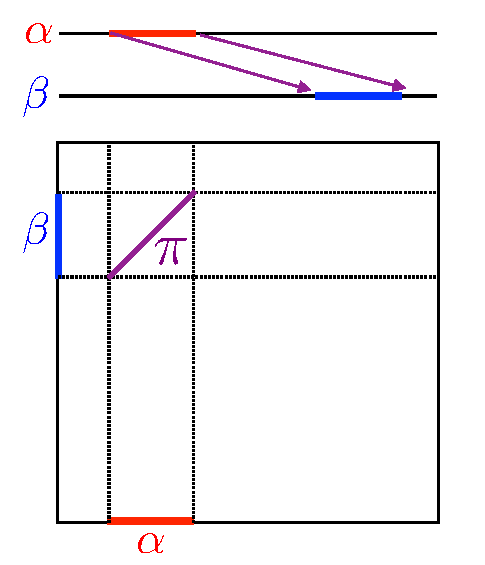
\includegraphics[width=.2\linewidth]{couplings/couplings-1}&
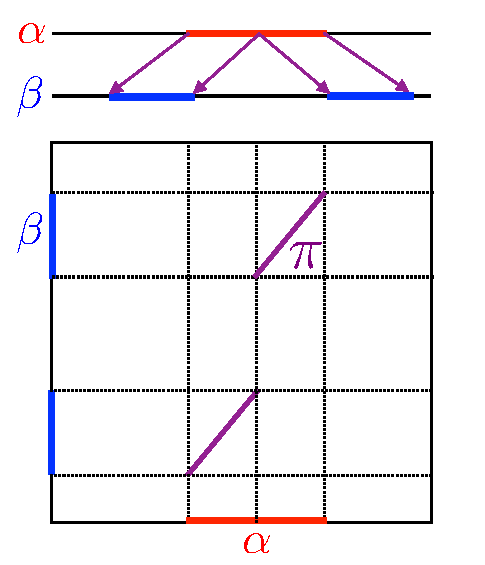
\includegraphics[width=.2\linewidth]{couplings/couplings-2}&
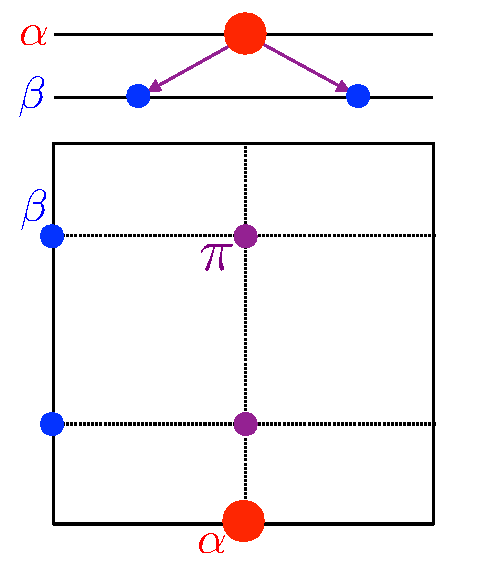
\includegraphics[width=.2\linewidth]{couplings/couplings-3}&
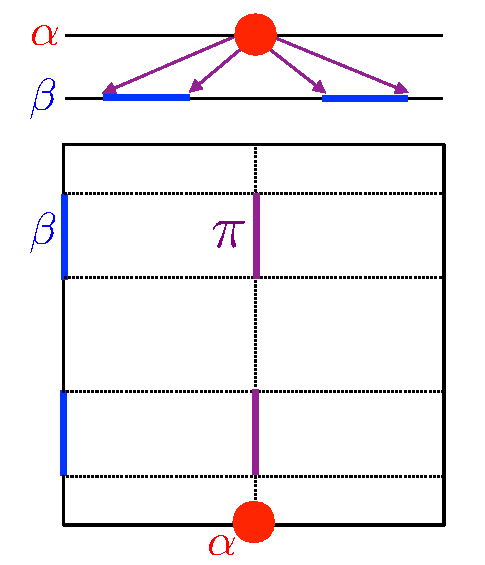
\includegraphics[width=.2\linewidth]{couplings/couplings-4}
\end{tabular}
\caption{\label{fig-couplings-simple}
Four simple examples of optimal couplings between 1-D distributions, represented as maps above (arrows) and couplings below. Inspired by~\cite{Levy2017review}.
}
\end{figure}


On compact domain $(\Xx,\Yy)$, \eqref{eq-mk-generic} always has a solution, because using the weak-* topology (so called weak topology of measures), the set of measure is compact, and a linear function with a continuous $c(x,y)$ is weak-* continuous. And the set of constraint is non empty, taking $\al \otimes \be$. On non compact domain, needs to impose moment condition on $\al$ and $\be$.




\todo{Brenier as Monge<=>Kanto}


%%%%%%%%%%%%%%%%%%%%%%%%%%%%%%%%%%%%%%%%%%%%%%%%%%%%%%%%%%%%%%%%%%%%%%%%%%%
\subsection{Metric Properties}


An important feature of OT is that it defines a distance between histograms and probability measures as soon as the cost matrix satisfies certain suitable properties. Indeed, OT can be understood as a canonical way to lift a ground distance between points to a distance between histogram or measures. 

We first consider the case where, using a term first introduce by~\cite{RubTomGui00}, the ``ground metric'' matrix $\C$ is fixed, representing substitution costs between bins, and shared across several histograms we would like to compare. The following proposition states that OT provides a meaningful distance between histograms supported on these bins.

\begin{prop}\label{prop-metric-histo}
We suppose $n=m$, and that for some $p \geq 1$, $\C=\distD^p=(\distD_{i,j}^p)_{i,j} \in \RR^{n \times n}$ where $\distD \in \RR_+^{n \times n}$ is a distance on $\range{n}$, \emph{i.e.}
\begin{enumerate}% [label=(\roman*)]
	\item $\distD \in \RR_+^{n \times n}$ is symmetric; 
	\item $\distD_{i,j}=0$ if and only if $i=j$; 
	\item $\foralls (i,j,k) \in \range{n}^3, \distD_{i,k} \leq \distD_{i,j}+\distD_{j,k}$.
\end{enumerate}
Then 
\eql{\label{eq-wass-p-disc}
	\WassD_p(\a,\b) \eqdef \MKD_{\distD^p}(\a,\b)^{1/p}
}
(note that $\WassD_p$ depends on $\distD$) defines the $p$-Wasserstein distance on $\Si_n$, \emph{i.e.} $\WassD_p$ is symmetric, positive, $\WassD_p(\a,\b)=0$ if and only if $\a = \b$, and it satisfies the triangle inequality
\eq{
	\foralls \a,\a',\b \in \Si_n, \quad \WassD_p(\a,\b) \leq \WassD_p(\a,\a') + \WassD_p(\a',\b).
}
\end{prop}

\begin{proof}
Symmetry and definiteness of the distance are easy to prove: since $\C = \distD^p$ has a null diagonal, $\WassD_p(\a,\a)=0$, with corresponding optimal transport matrix $\P^\star=\diag(\a)$; by the positivity of all off-diagonal elements of $\distD^p$, $\WassD_p(\a,\b)>0$ whenever $\a\ne \b$ (because in this case, an admissible coupling necessarily has a non-zero element outside the diagonal); by symmetry of $\distD^p$, $\WassD_p(\a,\b)=0$ is itself a symmetric function. 


To prove the triangle inequality of Wasserstein distances for arbitrary measures, \cite[Theorem 7.3]{Villani03} uses the gluing lemma, which stresses the existence of couplings with a prescribed structure. 
% Closed forms for such couplings exist in the discrete case which we can readily use. 
In the discrete setting, the explicit constuction of this glued coupling is simple.
%
Let $\a,\b,\VectMode{c} \in\simplex_n$. Let $\P$ and $\Q$ be two optimal solutions of the transport problems between $\a$ and $\b$, and $\b$ and $\VectMode{c}$ respectively. 
%
We define $\bar\b_j \eqdef \b_j$ if $\b_j>0$ and set otherwise $\bar\b_j=1$ (or actually any other value). We then define 
\eq{
	\SS \eqdef \P \diag(1/\bar\b) \Q \in \RR_+^{n \times n}.
} 
We remark that $\SS \in \U(\a,\VectMode{c})$ because 
\eq{
	\SS \ones_n  = \P \diag(1/\bar\b) \Q \ones_n = \P (\b / \bar\b) = \P \ones_{\Supp(\b)} = \a
}
where we denoted $\ones_{\Supp(\b)}$ the indicator of the support of $\b$, and we use the fact that $\P \ones_{\Supp(\b)} = \P \ones = \b$ because necessarily $\P_{i,j} = 0$ for $j \notin \Supp(\b)$.
Similarly one verifies that $\SS^\top \ones_n = \VectMode{c}$.


The triangle inequality follows from
%   notice that $\SS_{i\cdot k}$ being therefore a matrix of $\U(\a,\b)$ we can write:
$$\begin{aligned}
\WassD_p(\a,\VectMode{c})&=\left(\min_{\P\in U(\a,\VectMode{c})}\dotp{\P}{\distD^p}\right)^{1/p} \leq \dotp{\SS}{\distD^p}^{1/p}\\
&= \left(\sum_{ik} \distD^p_{ik}\sum_{j} \frac{\P_{ij}\Q_{jk}}{\bar\b_j}\right)^{1/p} \leq \left(\sum_{ijk} \left(\distD_{ij}+\distD_{jk}\right)^p \frac{\P_{ij}\Q_{jk}}{\bar\b_j}\right)^{1/p} \\
& \leq \left(\sum_{ijk} \distD^p_{ij} \frac{\P_{ij}\Q_{jk}}{\bar\b_j}\right)^{1/p} + \left(\sum_{ijk}\distD^p_{jk} \frac{\P_{ij}\Q_{jk}}{\bar\b_j}\right)^{1/p} \\
&= \left(\sum_{ij} \distD^p_{ij}\P_{ij} \sum_k \frac{\Q_{jk}}{\bar\b_j}\right)^{1/p} + \left(\sum_{jk} \distD^p_{jk} \Q_{jk} \sum_i \frac{\P_{ij}}{\bar\b_j}\right)^{1/p}\\
&= \left(\sum_{ij} \distD^p_{ij}\P_{ij}\right)^{1/p} + \left(\sum_{jk} \distD^p_{jk} \Q_{jk}\right)^{1/p}\\ 
&= \WassD_p(\a,\b) +\WassD_p(\b,\b).
\end{aligned}
$$
%
The first inequality is due to the suboptimality of $\SS$, the second is the usual triangle inequality for elements in $\distD$, and the third comes from Minkowski's inequality.
\end{proof}

Proposition~\ref{prop-metric-histo} generalizes from histogram to arbitrary measures that need not be discrete.

\begin{prop}\label{prop-metric-measure}
We assume $\X=\Y$, and that for some $p \geq 1$, $\c(x,y)=\dist(x,y)^p$ where $\dist$ is a distance on $\X$, \emph{i.e.} \\
	\hbox{}\qquad (i) $\dist(x,y) = \dist(y,x) \geq 0$;  \\
	\hbox{}\qquad (ii)  $\dist(x,y)=0$ if and only if $x=y$;  \\
	\hbox{}\qquad (ii)  $\foralls (x,y,z) \in \X^3, \dist(x,z) \leq \dist(x,y)+\dist(y,z)$. \\
Then 
\eql{\label{eq-defn-wass-dist}
	\Wass_p(\al,\be) \eqdef \MK_{\dist^p}(\al,\be)^{1/p}
}
(note that $\Wass_p$ depends on $\dist$) defines the $p$-Wasserstein distance on $\X$, \emph{i.e.} $\Wass_p$ is symmetric, positive, $\Wass_p(\al,\be)=0$ if and only if $\al = \be$, and it satisfies the triangle inequality
\eq{
	\foralls (\al,\be,\ga) \in  \Mm_+^1(\X)^3, \quad \Wass_p(\al,\ga) \leq \Wass_p(\al,\be) + \Wass_p(\be,\ga).
}
\end{prop}

\begin{proof}
The proof follows the same approach as that for Proposition~\ref{prop-metric-histo} and relies on the existence of a coupling between $(\al,\ga)$ obtained by ``guying'' optimal couplings between $(\al,\be)$ and $(\be,\ga)$.
\end{proof}

The Wasserstein distance $\Wass_p$ has many important properties, the most important one being that it is a weak distance, \emph{i.e.} it allows to compare singular distributions (for instance discrete ones) and to quantify spatial shift between the supports of the distributions. 
%
In particular, ``classical'' distances (or divergences) are not even defined between discrete distributions (the $L^2$ norm can only be applied to continuous measures with a density with respect to a base measure, and the discrete $\ell^2$ norm requires the positions $(x_i,y_j)$ to be fixed to work). In sharp contrast, one has that for any $p> 0$, $\Wass_p^p(\de_x,\de_y) = \dist(x,y)$. Indeed, it suffices to notice that $\Couplings(\de_x,\de_y)=\{ \delta_{x,y}\}$ and therefore the Kantorovich problem having only one feasible solution, $\Wass_p^p(\de_x,\de_y)$ is necessarily $(\dist(x,y)^p)^{1/p}=\dist(x,y)$. This shows that $\Wass_p(\de_x,\de_y) \rightarrow 0$ if $x \rightarrow y$. 
%
This property corresponds to the fact that $\Wass_p$ is a way to quantify the weak convergence as we now define. 

\begin{defn}[Weak convergence]\label{dfn-weak-conv}
	$(\al_k)_k$ converges weakly to $\al$ in $\Mm_+^1(\Xx)$ (denoted $\al_k \rightharpoonup \al$) if and only if for any continuous function $g \in \Cc(\Xx)$, $\int_\Xx g \d\al_k \rightarrow \int_\Xx g \d\al$.
	%
	This notion of weak convergence corresponds to the convergence in law of random vectors. 
\end{defn}

This convergence can be shown to be equivalent to $\Wass_p(\al_k,\al) \rightarrow 0$~\cite[Theorem 6.8]{Villani09} (together with a convergence of the moments up to order $p$ for unbounded metric spaces).

Note that there exists alternative distances which also metrize weak convergence. The simplest one are Hilbertian norms, defined as
\eq{
	\norm{\al}_k^2 \eqdef \EE_{\al \otimes \al}(k) = \int_{\X \times \X} k(x,y)\d\al(x)\d\al(y)
}
for a suitable choice of kernel $k : \X^2 \rightarrow \RR$. The most famous of such kernel is the Gaussian one $k(x,y)=e^{-\frac{\norm{x-y}^2}{2\si^2}}$ for some choice of bandwidth $\si>0$. 

This convergence should not be confounded with the strong convergence of measures, which is metrized by the TV norm $\norm{\al}_{TV} \eqdef |\al|(\X)$, which is the total mass of the absolute value of the measure.



\todo{rmk on gluying lemma}


%%%%%%%
\begin{rem}[Binary Cost Matrix and 1-Norm]\label{rem-binary}
One can easily check that when the cost matrix $\C$ is zero on the diagonal and $1$ elsewhere, namely when $\C=\ones_{n\times n}-I_n$, the OT distance between $\a$ and $\b$ is equal to the 1-norm of their difference, $\MKD_\C(\a,\b)=\norm{\a-\b}_1$.
%
One can also easily check that this result extends to discrete and discrete measures in the case where $c(x,y)$ is $0$ if $x=y$ and 1 when $x\ne y$. The OT distance between two discrete measures $\al$ and $\be$ is equal to their total variation distance.
\end{rem}
%%%%%%%




%%%%%
\paragraph{Case of Gaussians}

Bures metric, comparision with fisher-rao

\todo{Weak$^*$ metrization}

 comparison with TV
 
 
%%%%%
\paragraph{Applications and implications}

Applications for having a geometric distance : barycenters, shape registration loss functions, density fitting